\subsection{Diagramme afficher les menus
générés}\label{diagramme-afficher-les-menus-guxe9nuxe9ruxe9s}

\begin{figure}
\centering
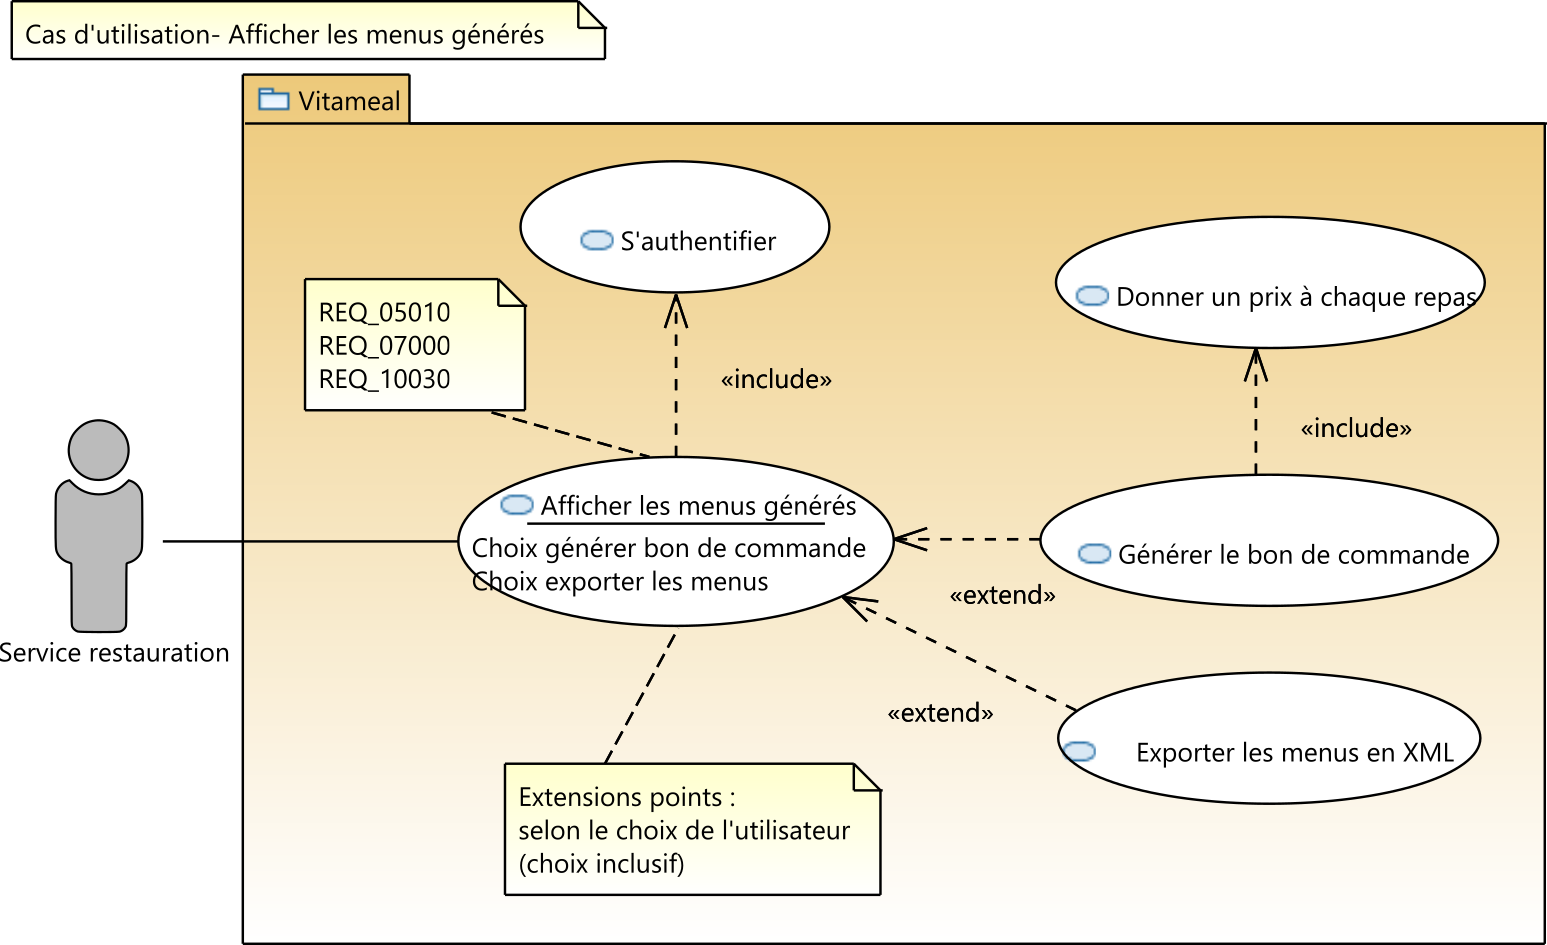
\includegraphics[width=0.85\textwidth]{../../CasDUtilisations/AfficherMenu/uc_afficher_menu.png}
\caption{Use case afficher les menus générés}
\end{figure}

\subsubsection{UC200 - Afficher les menus
générés}\label{uc200---afficher-les-menus-guxe9nuxe9ruxe9s}

\noindent\textbf{Nom :} Modifier un plat existant\\
\textbf{ID :} UC200\\
\textbf{Description :} Le service restauration souhaite pouvoir voir le
menu généré et selon son choix imprimer un bon\\
de commande et/ou exporter le menu sous un autre format.\\
\textbf{Auteur :} Nicolas SYMPHORIEN\\
\textbf{Dates(s) :} 08/05/2017\\
\textbf{Acteurs :} Le service restauration, par héritage, le diététicien
et le médecin\\
\textbf{Pré-condition :} L'utilisateur doit être identifié

\textbf{Scénario principal :}\\
1. Le système affiche un menu pour un groupe de patient donné 2.
L'utilisateur peut choisir de générer et voir le bon de commande associé
au menu affiché et l'utilisateur peut choisir de exporter le menu (pour
un usage par une tierce application)

\textbf{Scénario alternatif :}\\
1.a L'utilisateur peut changer de groupe de patient 1.b Le système
n'arrive pas à récupérer les menu générés 1.c Le système ne possède pas
de menu généré, il affiche un message d'information à l'utilisateur

\textbf{Post-Conditions:} Le menu est affiché. Un bon de commande est
produit. Un export est produit.

\subsubsection{UC201 - Générér le bon de
commande}\label{uc201---guxe9nuxe9ruxe9r-le-bon-de-commande}

\noindent\textbf{Nom :} Générer le bon de commande\\
\textbf{ID :} UC201\\
\textbf{Description :} Le service restauration souhaite pouvoir imprimer
un bon de commande du menu affiché\\
\textbf{Auteur :} Nicolas SYMPHORIEN\\
\textbf{Dates(s) :} 08/05/2017\\
\textbf{Acteurs :} Le service restauration, par héritage, le diététicien
et le médecin\\
\textbf{Pré-condition :} L'utilisateur doit être identifié

\textbf{Scénario principal :}\\
1. Le système propose la génération du menu si le prix de chaque plat a
été renseigné

\textbf{Scénario alternatif :}\\
1. a. Le prix de chaque plat n'a pas été renseigné

\textbf{Post-Conditions:} Le bon de commande et généré et affiché.

\subsubsection{UC202 - Donner un prix à chaque
repas}\label{uc202---donner-un-prix-uxe0-chaque-repas}

\noindent\textbf{Nom :} Donner un prix à chaque repas\\
\textbf{ID :} UC202\\
\textbf{Description :} Le service restauration souhaite pouvoir donnée
le pris de chaque plat composant un menu\\
\textbf{Auteur :} Nicolas SYMPHORIEN\\
\textbf{Dates(s) :} 08/05/2017\\
\textbf{Acteurs :} Le service restauration, par héritage, le diététicien
et le médecin\\
\textbf{Pré-condition :} L'utilisateur doit être identifié

\textbf{Scénario principal :}\\
1. Le système propose de renseigner le prix du plat

\textbf{Scénario alternatif :} aucun

\textbf{Post-Conditions:} Le prix du plat est renseigné

\subsubsection{UC203 - Exporter le menu affiché au format
XML}\label{uc203---exporter-le-menu-affichuxe9-au-format-xml}

\noindent\textbf{Nom :} Exporter le menu affiché au format XML\\
\textbf{ID :} UC203\\
\textbf{Description :} Le service restauration souhaite pouvoir exporté
le menu affiché pour un usage dans une tierce application (comme le site
internet de l'hopital par exemple)\\
\textbf{Auteur :} Nicolas SYMPHORIEN\\
\textbf{Dates(s) :} 08/05/2017\\
\textbf{Acteurs :} Le service restauration, par héritage, le diététicien
et le médecin\\
\textbf{Pré-condition :} L'utilisateur doit être identifié

\textbf{Scénario principal :}\\
1. Le système exporte le menu affiché en XML

\textbf{Scénario alternatif :} échec de l'export

\textbf{Post-Conditions:} Le menu est exportée au format XML
